\documentclass[crop,tikz]{standalone} 
\usepackage{tikz, amsmath, amssymb} 
\usetikzlibrary{positioning, shapes.geometric} 
\begin{document} 
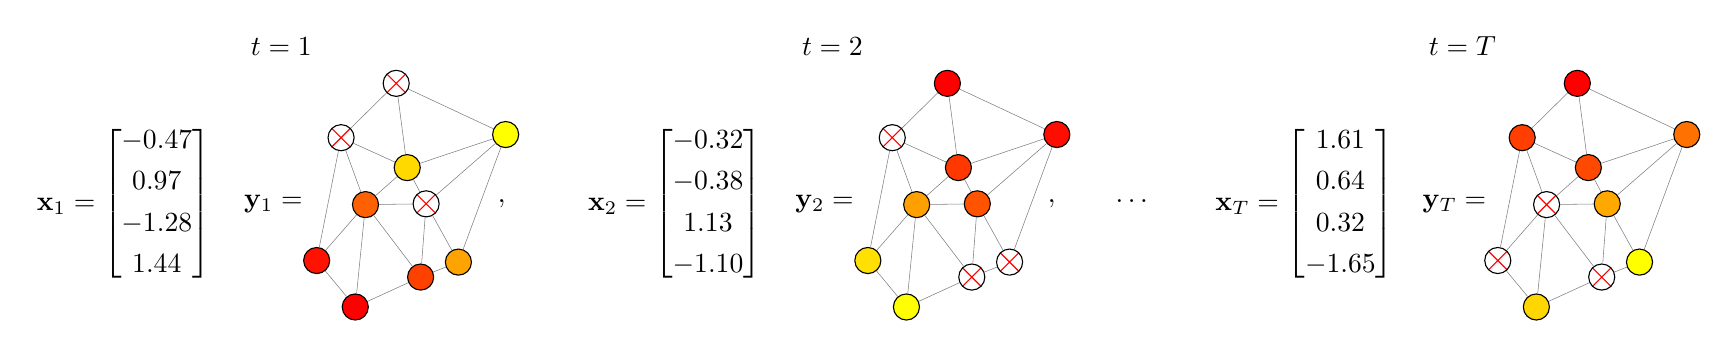
\begin{tikzpicture}[cross/.style={path picture={ 
    \draw[red]
  (path picture bounding box.south east) -- (path picture bounding box.north west) (path picture bounding box.south west) -- (path picture bounding box.north east);
  }}]

\draw (-1.5,2) node{$t = 1$}; 
\draw (-3.5,0) node{ $ \mathbf{x}_1 = \begin{bmatrix} -0.47 \\[0.1cm] 0.97 \\[0.1cm] -1.28 \\[0.1cm] 1.44 \end{bmatrix}$ };
\draw (-1.6,0) node{$\mathbf{y}_1 = $};

\node[circle, cross, draw, fill={rgb,255: red,255; green,255; blue,255}, minimum size=1mm] (0) at (0.34, -0.00) {};
\node[circle, draw, fill={rgb,255: red,255; green,255; blue,0}, minimum size=1mm] (1) at (1.35, 0.88) {};
\node[circle, draw, fill={rgb,255: red,255; green,18; blue,0}, minimum size=1mm] (2) at (-1.05, -0.72) {};
\node[circle, cross, draw, fill={rgb,255: red,255; green,255; blue,255}, minimum size=1mm] (3) at (-0.04, 1.53) {};
\node[circle, draw, fill={rgb,255: red,255; green,0; blue,0}, minimum size=1mm] (4) at (-0.56, -1.31) {};
\node[circle, cross, draw, fill={rgb,255: red,255; green,255; blue,255}, minimum size=1mm] (5) at (-0.74, 0.84) {};
\node[circle, draw, fill={rgb,255: red,255; green,97; blue,0}, minimum size=1mm] (6) at (-0.43, -0.01) {};
\node[circle, draw, fill={rgb,255: red,255; green,217; blue,0}, minimum size=1mm] (7) at (0.10, 0.46) {};
\node[circle, draw, fill={rgb,255: red,255; green,65; blue,0}, minimum size=1mm] (8) at (0.27, -0.93) {};
\node[circle, draw, fill={rgb,255: red,255; green,163; blue,0}, minimum size=1mm] (9) at (0.75, -0.74) {};

\draw[gray, very thin] (0) to (9);
\draw[gray, very thin] (0) to (8);
\draw[gray, very thin] (0) to (7);
\draw[gray, very thin] (0) to (6);
\draw[gray, very thin] (0) to (1);
\draw[gray, very thin] (1) to (9);
\draw[gray, very thin] (1) to (7);
\draw[gray, very thin] (1) to (3);
\draw[gray, very thin] (3) to (7);
\draw[gray, very thin] (3) to (5);
\draw[gray, very thin] (6) to (7);
\draw[gray, very thin] (5) to (6);
\draw[gray, very thin] (6) to (8);
\draw[gray, very thin] (2) to (5);
\draw[gray, very thin] (2) to (6);
\draw[gray, very thin] (2) to (4);
\draw[gray, very thin] (4) to (6);
\draw[gray, very thin] (4) to (8);
\draw[gray, very thin] (8) to (9);
\draw[gray, very thin] (7) to (5);

\draw (5.5,2) node{$t = 2$}; 
\draw (3.5,0) node{ $ \mathbf{x}_2 = \begin{bmatrix} -0.32 \\[0.1cm] -0.38 \\[0.1cm] 1.13 \\[0.1cm] -1.10 \end{bmatrix}$ };
\draw (5.4,0) node{$\mathbf{y}_2 = $};

\node[circle, draw, fill={rgb,255: red,255; green,83; blue,0}, minimum size=1mm] (10) at (7.34, -0.00) {};
\node[circle, draw, fill={rgb,255: red,255; green,13; blue,0}, minimum size=1mm] (11) at (8.35, 0.88) {};
\node[circle, draw, fill={rgb,255: red,255; green,224; blue,0}, minimum size=1mm] (12) at (5.95, -0.72) {};
\node[circle, draw, fill={rgb,255: red,255; green,0; blue,0}, minimum size=1mm] (13) at (6.96, 1.53) {};
\node[circle, draw, fill={rgb,255: red,255; green,255; blue,0}, minimum size=1mm] (14) at (6.44, -1.31) {};
\node[circle, cross, draw, fill={rgb,255: red,255; green,255; blue,255}, minimum size=1mm] (15) at (6.26, 0.84) {};
\node[circle, draw, fill={rgb,255: red,255; green,160; blue,0}, minimum size=1mm] (16) at (6.57, -0.01) {};
\node[circle, draw, fill={rgb,255: red,255; green,56; blue,0}, minimum size=1mm] (17) at (7.10, 0.46) {};
\node[circle, cross, draw, fill={rgb,255: red,255; green,255; blue,255}, minimum size=1mm] (18) at (7.27, -0.93) {};
\node[circle, cross, draw, fill={rgb,255: red,255; green,255; blue,255}, minimum size=1mm] (19) at (7.75, -0.74) {};

\draw[gray, very thin] (10) to (19);
\draw[gray, very thin] (10) to (18);
\draw[gray, very thin] (10) to (17);
\draw[gray, very thin] (10) to (16);
\draw[gray, very thin] (10) to (11);
\draw[gray, very thin] (11) to (19);
\draw[gray, very thin] (11) to (17);
\draw[gray, very thin] (11) to (13);
\draw[gray, very thin] (13) to (17);
\draw[gray, very thin] (13) to (15);
\draw[gray, very thin] (16) to (17);
\draw[gray, very thin] (15) to (16);
\draw[gray, very thin] (16) to (18);
\draw[gray, very thin] (12) to (15);
\draw[gray, very thin] (12) to (16);
\draw[gray, very thin] (12) to (14);
\draw[gray, very thin] (14) to (16);
\draw[gray, very thin] (14) to (18);
\draw[gray, very thin] (18) to (19);
\draw[gray, very thin] (17) to (15);

\draw (13.5,2) node{$t = T$}; 
\draw (11.5,0) node{ $ \mathbf{x}_T = \begin{bmatrix} 1.61 \\[0.1cm] 0.64 \\[0.1cm] 0.32 \\[0.1cm] -1.65 \end{bmatrix}$ };
\draw (13.4,0) node{$\mathbf{y}_T = $};

\node[circle, draw, fill={rgb,255: red,255; green,169; blue,0}, minimum size=1mm] (20) at (15.34, -0.00) {};
\node[circle, draw, fill={rgb,255: red,255; green,113; blue,0}, minimum size=1mm] (21) at (16.35, 0.88) {};
\node[circle, cross, draw, fill={rgb,255: red,255; green,255; blue,255}, minimum size=1mm] (22) at (13.95, -0.72) {};
\node[circle, draw, fill={rgb,255: red,255; green,0; blue,0}, minimum size=1mm] (23) at (14.96, 1.53) {};
\node[circle, draw, fill={rgb,255: red,255; green,214; blue,0}, minimum size=1mm] (24) at (14.44, -1.31) {};
\node[circle, draw, fill={rgb,255: red,255; green,62; blue,0}, minimum size=1mm] (25) at (14.26, 0.84) {};
\node[circle, cross, draw, fill={rgb,255: red,255; green,255; blue,255}, minimum size=1mm] (26) at (14.57, -0.01) {};
\node[circle, draw, fill={rgb,255: red,255; green,73; blue,0}, minimum size=1mm] (27) at (15.10, 0.46) {};
\node[circle, cross, draw, fill={rgb,255: red,255; green,255; blue,255}, minimum size=1mm] (28) at (15.27, -0.93) {};
\node[circle, draw, fill={rgb,255: red,255; green,255; blue,0}, minimum size=1mm] (29) at (15.75, -0.74) {};

\draw[gray, very thin] (20) to (29);
\draw[gray, very thin] (20) to (28);
\draw[gray, very thin] (20) to (27);
\draw[gray, very thin] (20) to (26);
\draw[gray, very thin] (20) to (21);
\draw[gray, very thin] (21) to (29);
\draw[gray, very thin] (21) to (27);
\draw[gray, very thin] (21) to (23);
\draw[gray, very thin] (23) to (27);
\draw[gray, very thin] (23) to (25);
\draw[gray, very thin] (26) to (27);
\draw[gray, very thin] (25) to (26);
\draw[gray, very thin] (26) to (28);
\draw[gray, very thin] (22) to (25);
\draw[gray, very thin] (22) to (26);
\draw[gray, very thin] (22) to (24);
\draw[gray, very thin] (24) to (26);
\draw[gray, very thin] (24) to (28);
\draw[gray, very thin] (28) to (29);
\draw[gray, very thin] (27) to (25);

\draw (1.3, 0) node{$,$}; 
 \draw (8.9, 0) node{$, \quad\quad \dots $};

\end{tikzpicture}
\end{document} 
